\documentclass[12pt, letterpaper]{article} %letterpaper is 8.5 x 11
\usepackage[english]{babel} %different lanuages, choose english rules
\usepackage[utf8]{inputenc} %begone utf 16
\usepackage{graphicx} %to insert images
\graphicspath{ {images/} } %path containing images
\usepackage{fancyhdr} %for headers and footers

\pagestyle{fancy} %use fancyhdr
\fancyhf{}

%heading on every page
\lhead{Discrete Homework}
\rhead{Khinshan Khan}
%footer numbers
\fancyfoot[C]{\thepage} % except the center


\begin{document}
\section{} %we can use section as the question number
A connected planar graph has 6 vertices and 8 edges.  How many faces
does it have?  Draw an example of such graph.
\\*
\\ %start a new paragraph
BRIEF WORK HERE??
\\* %start a new line but not a new paragraph

%if need be, an image
\begin{figure}[h]
  \centering
  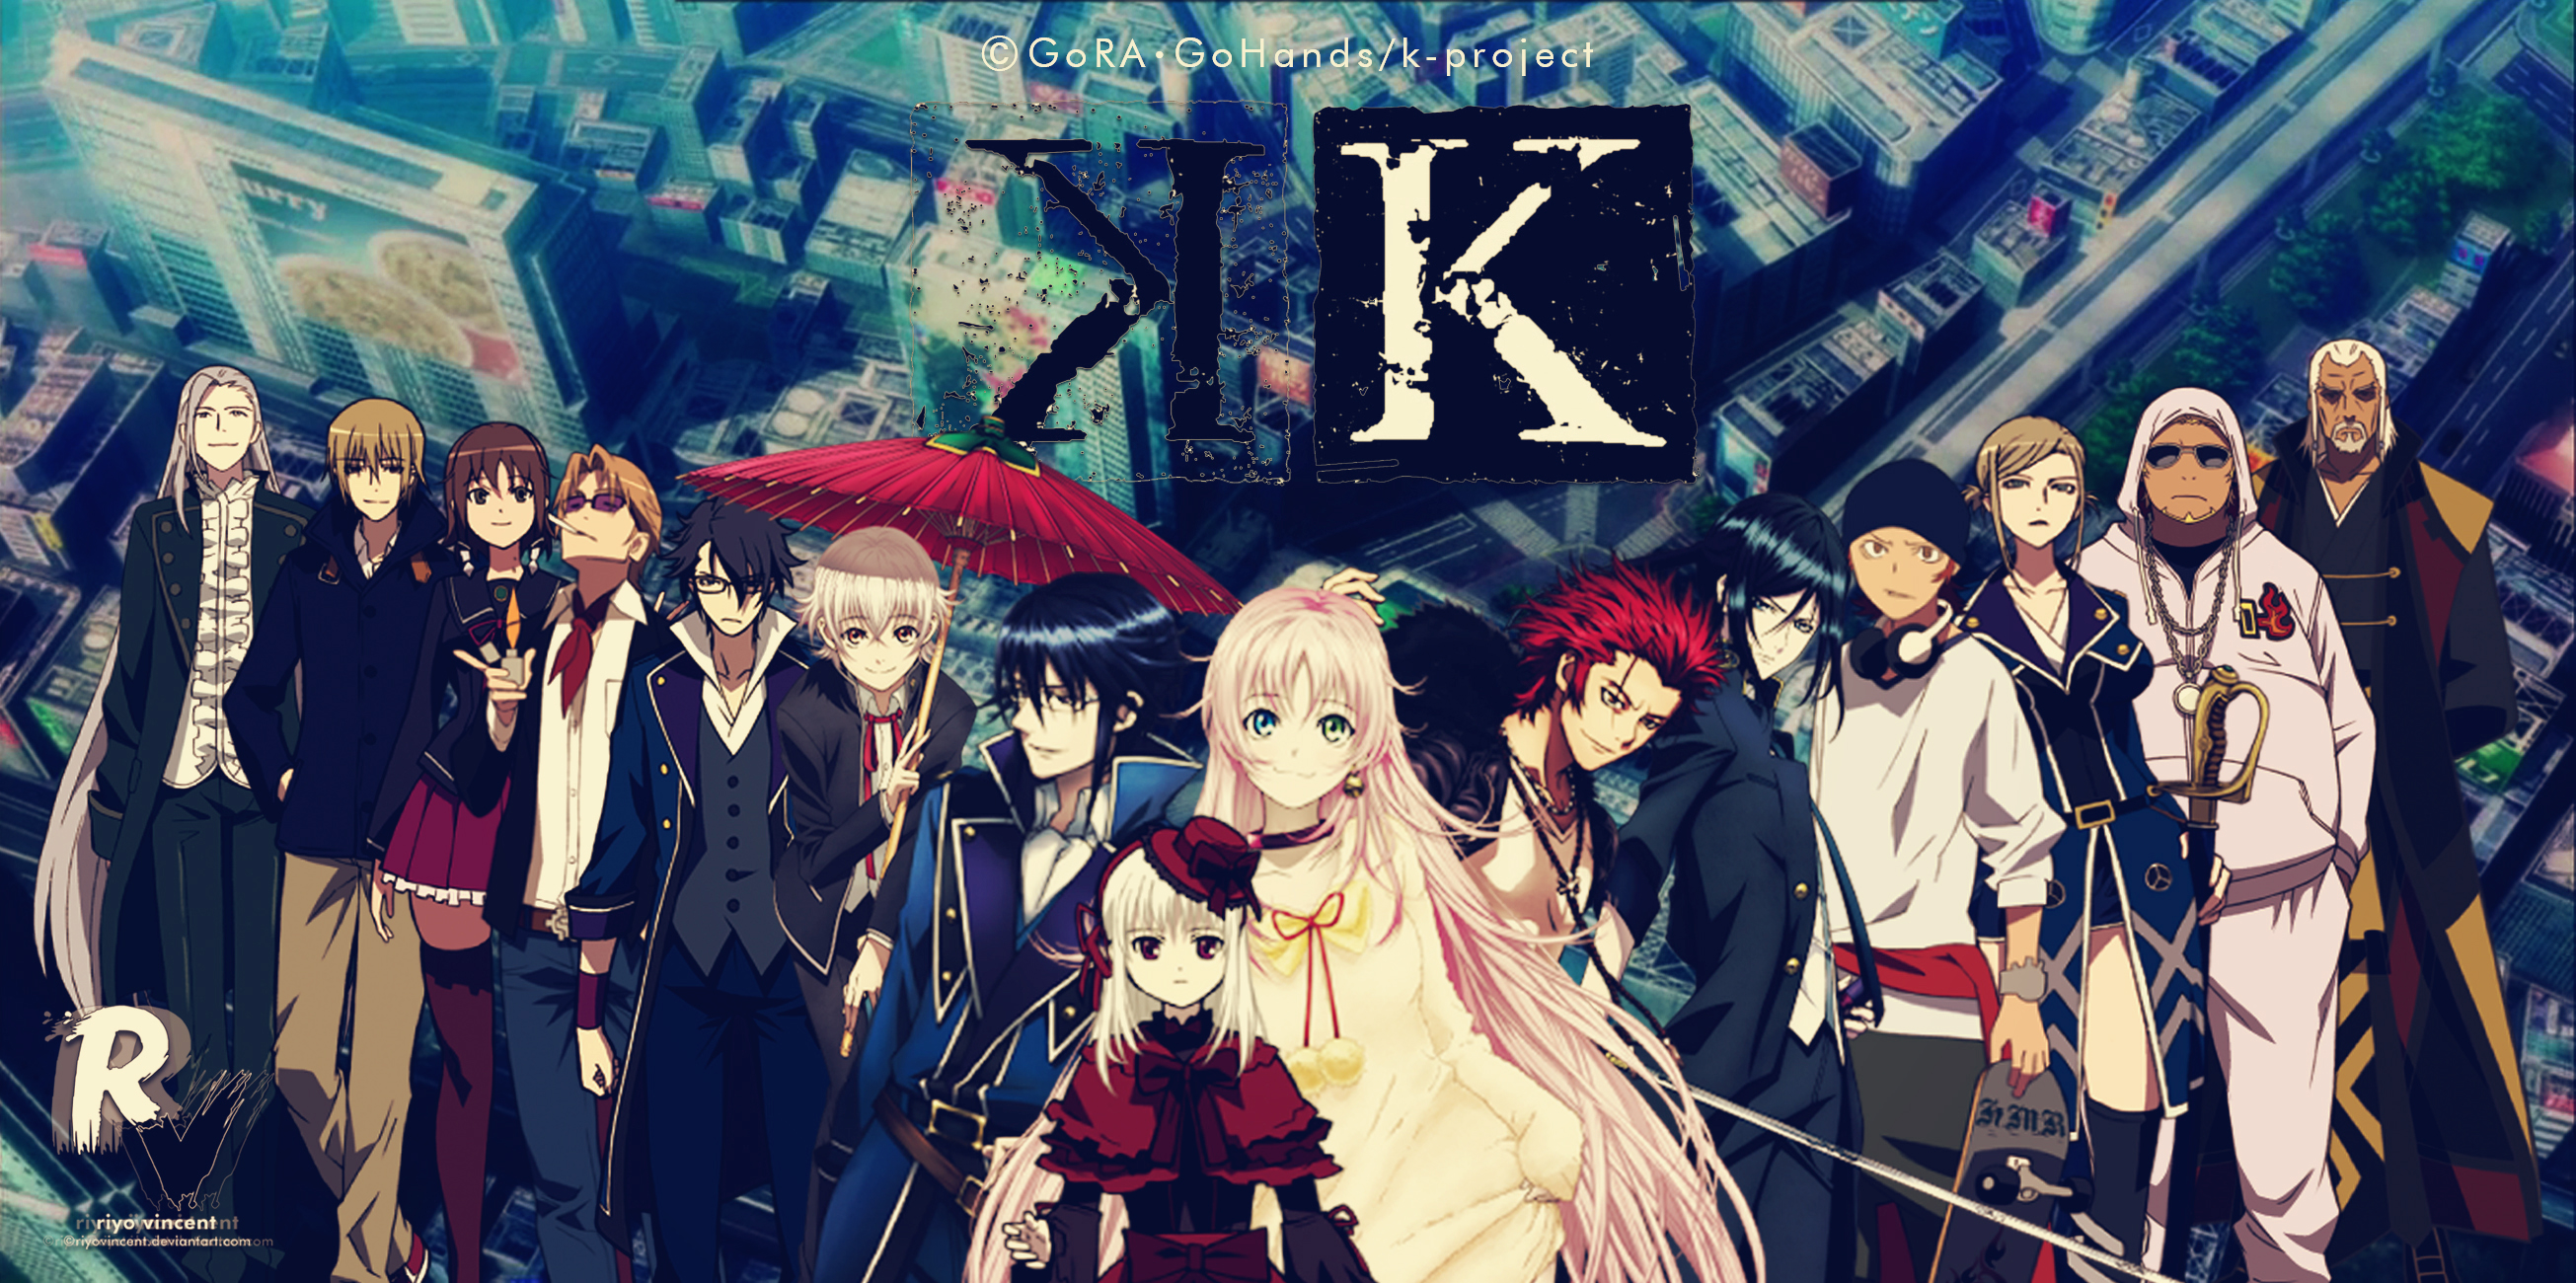
\includegraphics[width=\linewidth]{image1}
  \caption{K Project}
  \label{fig:wholesome}
\end{figure}

%more text
\noindent CONTINUED WORK??
\\
this is a ref to the image: \ref{fig:wholesome}

\pagebreak %start a new page
\section{}
In how many ways can we stack 10 books?
\\ %start a new paragraph
\\*
Answer: We are looking for the number of different ways to order the books, which is 10!. This combination is equal to $\prod_{i=1}^{10} i $, which evaluates to 3628800. Ergo, there are 3628800 ways to stack 10 books.
\end{document}
